
\chapter{Recomendaciones para mejorar la performance de Javascript}
Las aplicaciones web de la actualidad utilizan una gran cantidad de codigo Javascript, en particular algunas utlizan Javascript para ejecutar gran parte de la
interfaz de usuario. Como resultado se tienen varias lineas de código que se ejecutan cada vez que el usuario interactúa con la página. Por lo tanto la performance
no sólo involucra el tiempo en que tarda la página en cargar, sino también como responde la interfaz de usuario al ser utilizada.

\section{Scope}
Cuando se ejecuta código Javascript, se crea un contexto de ejecución (denominado \emph{scope}). El contexto de ejecución define el entorno en el cual el código es
ejecutado. Un contexto de ejecución global es creado al cargar la página, contextos adicionales son creados para cada función que se ejecuta, por lo que se crea
un \emph{stack} de contextos de ejecución, en el cual el que se encuentra al comienzo, es el contexto de ejecución activo.

Cada contexto de ejecución tiene una \emph{scope chain} asociada, que es utilizada para la resolución de identificadores. La \emph{scope chain} contiene uno o más
objetos que definen identificadores para el contexto de ejecución. El contexto de ejecución global tiene un sólo objeto variable en su \emph{scope chain}, el cual define
todas las variables globales y funciones disponibles en Javascript.

Cuando una función es creada pero no ejecutada, su propiedad interna [[Scope]] contiene la \emph{scope chain} del contexto de ejecución en el cual fue creada. En
cuanto el flujo de ejecución entra en una función, un ``objeto de activación'' es creado e inicializado con valores para \emph{this}, \emph{arguments}, \emph{named arguments}
y las variables locales correspondientes a la función. El objeto de activaciones ubicado al comienzo de la \emph{scope chain} del contexto de ejecución es seguido por
los objetos contenidos en la propiedad [[Scope]] de la función.

Durante la ejecución, los identificadores como los nombres de las funciones y variables son resueltos buscando en la \emph{scope chain} del contexto de ejecución. La resolución
de identificadores comienza al principio de la \emph{scope chain}. Consideremos el siguiente ejemplo de código:

\begin{em}
function add(num1, num2)\{
    return num1 + num2;
\}

var result = add(5, 10);
\end{em}

Cuando éste código es ejecutado, la función add tiene una propiedad [[Scope]] que solo contiene al objeto global. En el momento en que el flujo de ejecución entra en la función
suma, un nuevo contexto de ejecución es creado, y un objeto de activación, conteniendo \emph{this}, \emph{arguments}, \emph{num1}, y \emph{num2} es ubicado al comienzo
de la \emph{scope chain}.

\begin{figure}[h]
\centering
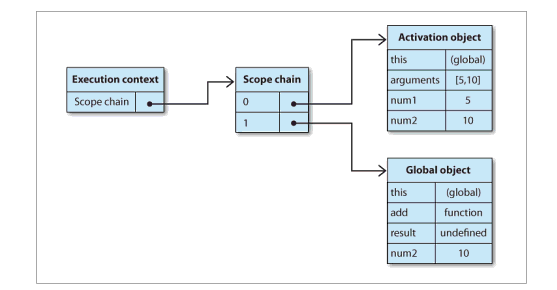
\includegraphics[width=1\textwidth]{figuras/scope_chain.png}
	\caption{Relación entre el contexto de ejecución y la \emph{scope chain}}
    \label{fig.scope_chain}
\end{figure}

Dentro de la función add, los identificadores \emph{num1} y \emph{num2} deben ser resueltos cuando la función esta ejecutando. Esta resolución se lleva a cabo inspeccionando
cada objeto en la \emph{scope chain} hasta que el identificador es encontrado. La búsqueda comienza con el primer elemento de la \emph{scope chain}, el cual es el registro
de activación que contiene las variables locales de la función. Si el identificador no es encontrado, el siguiente objeto de la \emph{scope chain} es inspeccionado en busca del
identificador.

Entender cómo funcionan los \emph{scopes} y las \emph{scope chain} en Javascript es importante, debido a que la performance de la resolución de identificadores esta directamente
relacionada al numero de objetos en la \emph{scope chain}.

\section{Variables locales}

Las variables locales son por lejos los identificadores más rápidos en los cuales se puede escribir y leer. Debido a que existen en los objetos de activación de la función
en ejecución, la resolución de identificadores involucra la inspección de un sólo objeto en la \emph{scope chain}. La cantidad de tiempo necesaria para leer el valor de una
variable aumenta con cada elemento que haya que inspeccionar en la \emph{scope chain}. Como las variables locales son las que se encuentran al comienzo de la \emph{scope chain}
son las mas rápidas de acceder, y por lo tanto es una buena práctica almacenar en variables locales todas las variables globales que sean referenciadas más de una vez
dentro de una función.

\section{La sentencia with}
La \emph{scope chain} para cierto contexto de ejecución normalmente no cambia durante la ejecución del código. Existen dos sentencias que temporalmente incrementan la
\emph{scope chain} de un contexto de ejecución. La primera es la sentencia with, que fue diseñada para permitir un acceso más simple a las propiedades de un objeto haciéndolas
parecer variables locales. Por ejemplo:

\begin{em}
var person = \{
    name: ``Nicholas'',
    age: 30
\};

function displayInfo()\{
    var count = 5;
    with(person)\{
        alert(name + `` is '' + age);
        alert(``Count is '' + count);
    \}
\}

displayInfo();
\end{em}

En esta función, el objeto \emph{person} es pasado en un bloque \emph{with}. Esto permite el acceso a las propiedades \emph{name} y \emph{age} como si hubieran sido definidas
de manera local. Lo que en verdad ocurre, es que un nuevo objeto es agregado al comienzo de la \emph{scope chain} del actual contexto de ejecucion.

\begin{figure}[h]
\centering
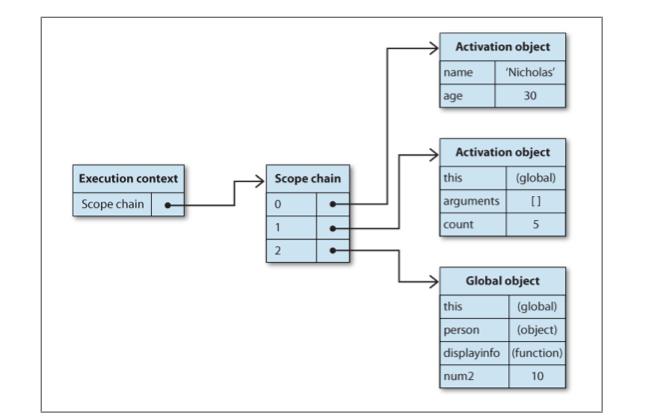
\includegraphics[width=1\textwidth]{figuras/scope_chain_with_statement.png}
	\caption{\emph{Scope chain} al utilizar la sentencia with}
    \label{fig.scope_chain_with_statement}
\end{figure}

Si bien el uso de esta sentencia puede parecer muy conveniente cuando las propiedades de un objeto son utilizadas con mucha frecuencia, este objeto extra en la
\emph{scope chain} del contexto daña la performance de la resolución de identificadores, debido a que las variables locales de la función pasan a encontrarse en el segundo
objeto en la \emph{scope chain}.

La sentencia \emph{catch} (correspondiente al bloque \emph{try catch}) es la segunda sentencia que aumenta el tamaño de la \emph{scope chain}. Ésta se comporta de manera
similar a la sentencia \emph{with} al agregar un objeto al comienzo de la \emph{scope chain} mientras ejecuta el código dentro del bloque. Ese objeto contiene una entrada
para la excepción especificada en la sentencia \emph{catch}. Sin embargo la sentencia \emph{catch} es ejecutada sólo cuando ocurre un error durante la ejecución de la
sentencia \emph{try}, resultando menos problemática que la snetencia \emph{with}.

